\documentclass[conference]{IEEEtran}
\IEEEoverridecommandlockouts
% The preceding line is only needed to identify funding in the first footnote. If that is unneeded, please comment it out.
\usepackage{cite}
\usepackage{amsmath,amssymb,amsfonts}
\usepackage{algorithmic}
\usepackage{graphicx}
\usepackage{textcomp}
\usepackage{xcolor}
\usepackage{float}
\usepackage{booktabs}
\raggedbottom
\def\BibTeX{{\rm B\kern-.05em{\sc i\kern-.025em b}\kern-.08em
    T\kern-.1667em\lower.7ex\hbox{E}\kern-.125emX}}


\begin{document}

\title{Detail in Context: A Multi-Scale and Clinical Machine Learning Framework for Mycosis Fungoides Detection
}

\author{
    \IEEEauthorblockN{Anonymous Author(s)}
    \vspace{0.15cm}
    \IEEEauthorblockA{\textit{Affiliation omitted for double-blind review}}
}

\maketitle

\begin{abstract}
    Mycosis fungoides (MF) is a rare form of cutaneous T-cell lymphoma that is often misdiagnosed 
    in early stages due to its visual similarity to benign inflammatory dermatoses. 
    Early and accurate diagnosis is critical for improving patient outcomes. 
    In this paper, we propose a comprehensive diagnostic framework for automated MF detection 
    that integrates multi-scale histopathological image analysis with a machine learning-based clinical classifier. 
    The proposed approach leverages dual-magnification (10$\times$ and 20$\times$) convolutional neural networks (CNNs) 
    in a late-fusion ensemble to distinguish MF from other lymphoproliferative skin conditions, 
    complemented by a Random Forest classifier analyzing 16 clinical features. 
    Experimental results on an expanded dataset of 6,257 images (4,296 MF; 1,961 Non-MF) across 463 patients 
    demonstrate that prioritizing cytological details (20$\times$) within broader architectural context (10$\times$) yields strong 
    performance. The image-based late-fusion model achieves an accuracy of 83.58\% and a sensitivity of 89.13\%, 
    while the clinical Random Forest model achieves an accuracy of 96.6\% and sensitivity of 93.8\%, 
    highlighting the potential of this multimodal framework as a robust clinical decision support system.
\end{abstract}

\begin{IEEEkeywords}
    Mycosis Fungoides, Deep Learning, Histopathology, Medical Image Analysis, Clinical Decision Support System
\end{IEEEkeywords}
% =====================
% 1. Introduction
% =====================
\section{Introduction}
Mycosis Fungoides (MF) is a type of skin lymphoma characterized by malignant proliferation of skin-homing T
lymphocytes and is considered the most common primary cutaneous lymphoma (CL), making up almost 50\% of all cases \cite{willemze2005}. Despite its prevalence among utaneous
T-cell lymphomas (CTCLs), MF remains a rare disease with an estimated incidence of 0.5 cases per 100,000 person-years \cite{willemze2005}.
The clinical presentation of MF is highly variable, often manifesting as erythematous patches, plaques, or tumors that can easily be mistaken for
benign inflammatory skin conditions such as eczema or psoriasis. This diagnostic ambiguity contributes to significant delays in accurate diagnosis,
with studies reporting an average time to diagnosis of 3-6 years from symptom onset \cite{beatty2025_early_mf_diagnosis}.
MF remains challenging to diagnose, particularly in early stages, where clinical presentations often mimic benign skin disorders such as eczema or psoriasis.

Recent advances in deep learning have shown significant promise in medical image
analysis \cite{litjens2017deep}, particularly in dermatology \cite{esteva2017dermatologist}.
However, most existing studies
focus on common skin cancers such as melanoma, while rare diseases like MF remain underexplored. This work aims to address this gap by developing and evaluating a
deep-learning-based system for MF detection in histopathological skin images.

The main contributions of this work can be summarized as follows:
\begin{itemize}
    \item A multi-scale MF modeling approach leveraging TF-EfficientNet-B3 architectures trained on histopathological images at 10$\times$ and 20$\times$ magnifications.
    \item A patient-level MF detection strategy based on mean aggregation of patch-level probabilities.
    \item A weighted late-fusion model integrating multi-magnification decisions that explicitly prioritizes cytological cellular details over low-power architectural context to maximize sensitivity.
    \item A robust machine learning-based clinical classifier evaluating 16 patient metadata features, rigorously compared across XGBoost, Random Forest, and Logistic Regression algorithms to serve as a complementary diagnostic signal.
\end{itemize}

% =====================
% 2. Related Work
% =====================
\section{Related Work}
Previous research in dermatological image analysis has primarily focused on melanoma detection and benign-versus-malignant lesion classification.
Studies employing convolutional neural networks (CNNs) have demonstrated dermatologist-level performance in some tasks \cite{Doeleman2024-MF}.
However, literature addressing MF specifically remains limited, largely due to dataset scarcity, subtlety  of  histopathological features,
and high inter-observer variability.

Recent works have explored AI-based approaches for lymphoproliferative skin diseases, yet MF is often excluded or significantly underrepresented, underscoring the
need for targeted investigation into AI-assisted MF diagnosis.

Almost all recent studies rely on digitized whole-slide images (WSIs) for histopathological analysis. In contrast, to address the lack of digital slide
scanners prevalent in resource-limited countries, our framework operates on conventional microscopic images acquired at fixed magnifications rather than WSIs.
This setting reflects real-world clinical constraints and represents a novel direction that is largely absent from recent literature.
Contemporary approaches predominantly employ weakly supervised deep learning frameworks, such as clustering-constrained attention multiple instance
learning (CLAM) \cite{Lu2021} or toolkits such as Trident \cite{zhang2025standardizing, vaidya2025molecular}, which are designed to leverage WSIs.
Our approach diverges from these paradigms by focusing on magnification-specific image analysis under practical acquisition conditions.


% =====================
% 3. Materials and Methods
% =====================
\section{Materials and Methods}

\subsection{Dataset}
The dataset used in this study was collected through a clinical collaboration with the 
dermatopathology unit of a major tertiary care university hospital.
It consists of retrospective histopathological images captured from regions of interest with 
salient histopathological features discernible to a junior dermatologist, as well as associated clinical metadata. 
The dataset comprises images from a total of 463 unique patients, yielding 6,257 images in total.

Cases were categorized into two primary classes: Mycosis Fungoides (MF) and non-MF. 
The MF cohort includes 310 patients (4,296 images), while the non-MF cohort comprises 
153 patients (1,961 images) spanning other lymphoproliferative skin disorders, including 
B-cell lymphoma (358 images, 18 patients), pityriasis lichenoides et varioliformis acuta 
and chronica (PLEVA/PLC) (1,268 images, 108 patients), T-cell dyscrasia 
(180 images, 15 patients), and pseudolymphoma (155 images, 11 patients). 
This heterogeneous non-MF group reflects real-world diagnostic challenges encountered 
in clinical practice.

The dataset was partitioned at the patient level into training, validation, and 
test sets to prevent data leakage. The split consisted of 329 training patients, 67 validation patients, and 67 test patients. 
The acquired images were subsequently processed into patches for deep learning model training. 
The 20$\times$ dataset consisted of 23,062 training patches, 4,728 validation patches, and 4,320 test patches, 
while the 10$\times$ dataset comprised 73,824 training patches, 14,804 validation patches, and 12,848 test patches.

Due to the private nature of the dataset and institutional constraints, the images are not publicly available.


\subsection{Preprocessing}
All input images were provided in \texttt{.tif} format and acquired at a native resolution of $2560 \times 1920$ pixels. 
The images were hematoxylin and eosin (H\&E) stained and captured at fixed optical magnifications.
We used a sliding window approach to extract diagnostically relevant patches. 
To capture appropriate spatial context, the extraction parameters were tailored to the optical magnification:
\begin{itemize}
    \item \textbf{10$\times$ Magnification:} $512 \times 512$ pixel patches with a stride of 256 pixels (50\% overlap).
    \item \textbf{20$\times$ Magnification:} $1024 \times 1024$ pixel native patches (subsequently resized to $512 \times 512$ for network input) with a stride of 512 pixels.
\end{itemize}

Foreground extraction was applied to remove non-informative background regions prior to model training. 
An initial attempt based on conventional RGB thresholding—implemented by converting images to grayscale and applying a 
mean-intensity threshold—proved insufficient due to staining variability and inconsistent background illumination. 
Consequently, a more robust strategy was adopted by converting patches to the HSV color space and filtering background 
regions based on saturation values. Specifically, the proportion of pixels with saturation greater than a predefined 
threshold was computed for each patch, and patches with insufficient foreground content were discarded as shown in 
Figure \ref{fig:HSV_Ratio}. A minimum foreground ratio of 0.285 was enforced, effectively suppressing background-dominated 
patches while preserving diagnostically relevant tissue regions.

Data augmentation was applied exclusively to the training set to improve generalization and mitigate class imbalance. 
Given the orientation-invariant nature of histopathological features, spatial transformations played a central role. 
These included random horizontal and vertical flipping, as well as random rotations within a limited angular range. 
Additional photometric augmentations, such as controlled variations in brightness, contrast, saturation, and hue, were 
introduced to account for staining and acquisition variability. Following augmentation, patches were converted to tensor 
representations and normalized using ImageNet statistics to align with pretrained network initialization.
\begin{figure}
    \centering
    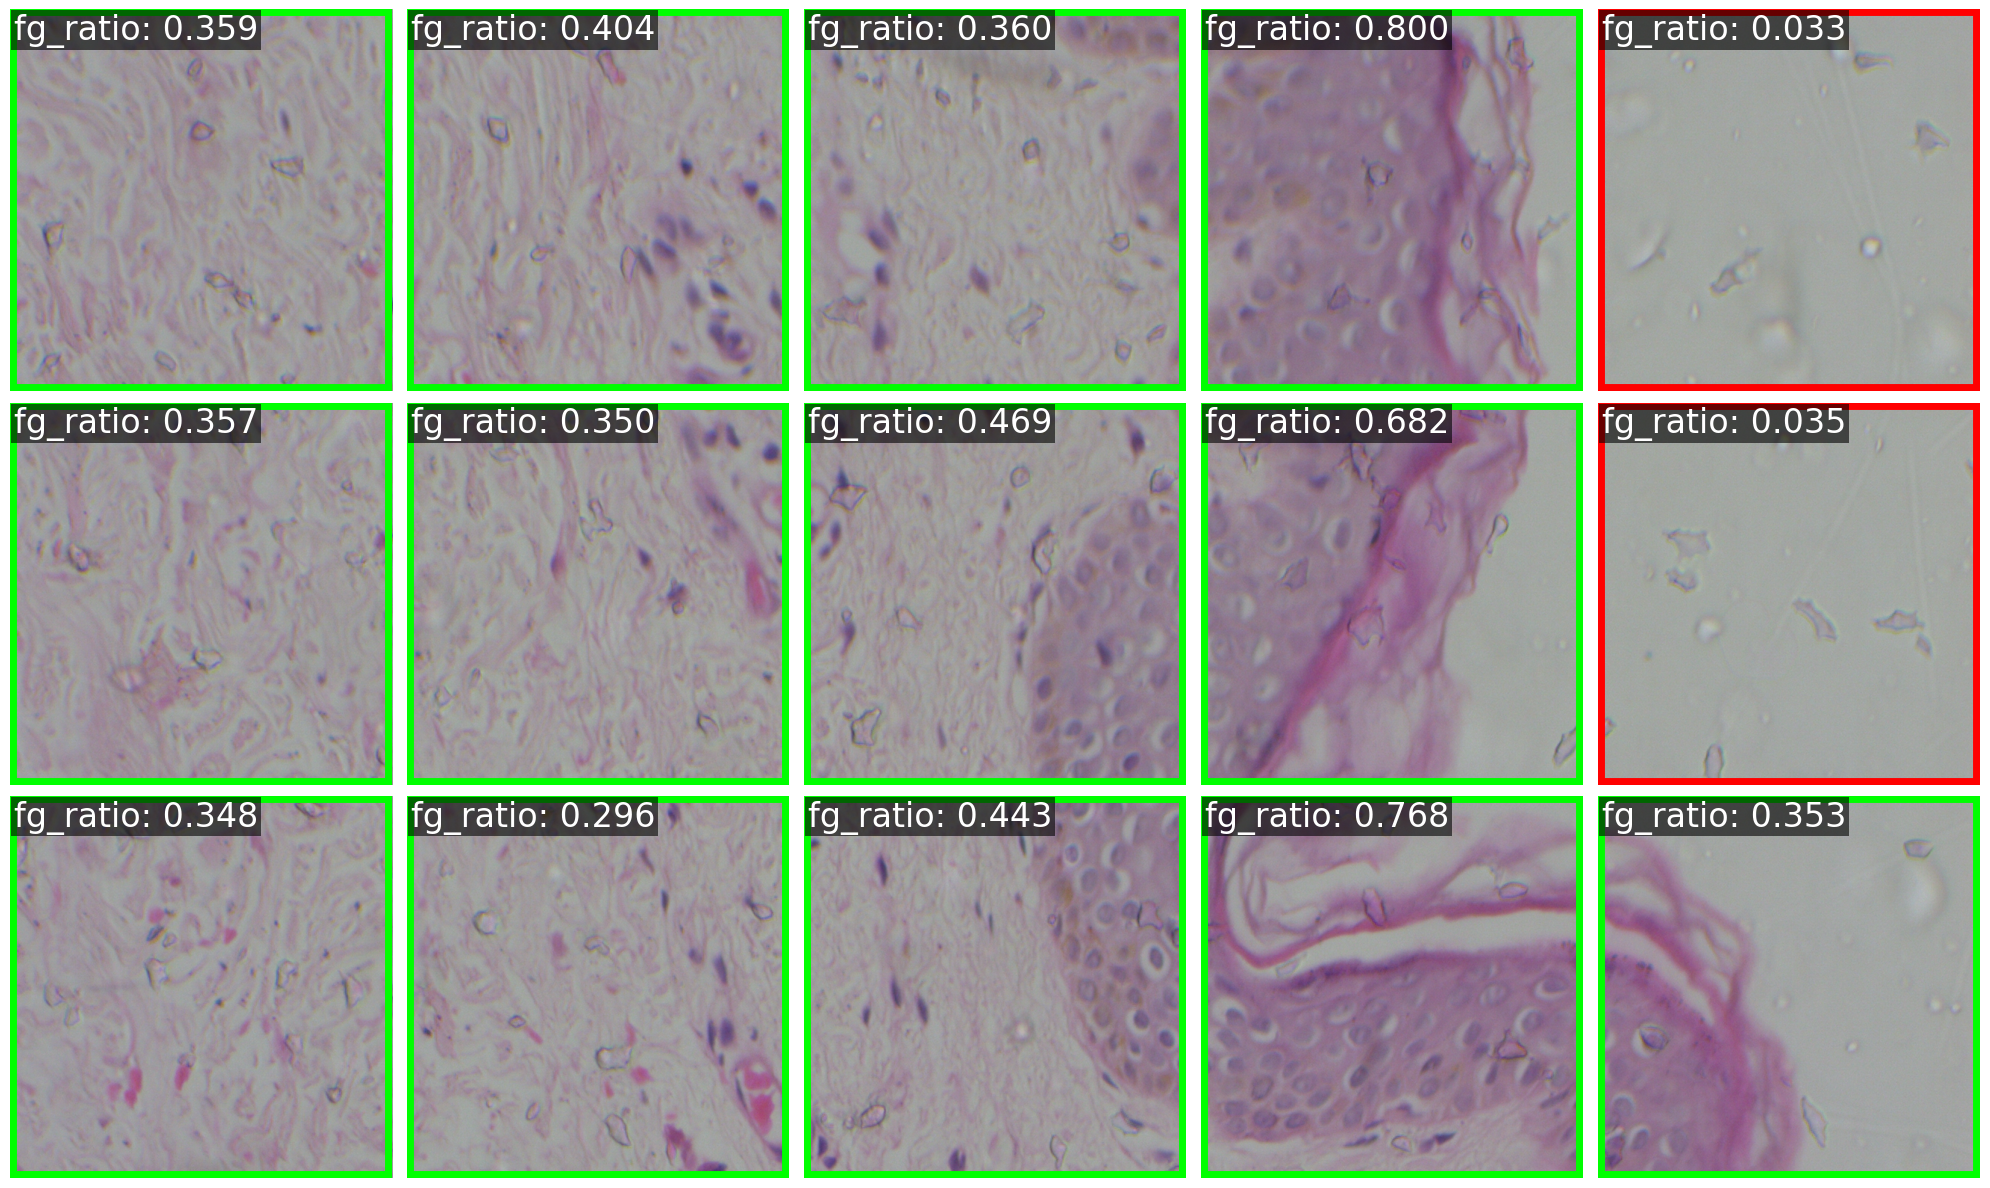
\includegraphics[width=1\linewidth]{HSV_Ratio.png}
    \caption{Different foreground ratios for patches of a sample tif image}
    \label{fig:HSV_Ratio}
\end{figure}

\subsection{Model Architecture and Training Protocol}

\subsubsection{Dual-Magnification Architecture}
To capture both broad architectural distortion and granular cellular atypia, we deployed a 
two-branch architecture utilizing independent feature extractors. Both models leverage the 
\textbf{TF-EfficientNet-B3} backbone (approximately 10.3M parameters) to distinguish between 
5 target classes (MF, PLEVA-PLC, Pseudolymphoma, T-cell dyscrasia, and B-cell Lymphoma). 
The configurations for each magnification are summarized in Table \ref{tab:hyperparams}.

\begin{table}[htbp]
\caption{Model Configuration and Hyperparameters}
\label{tab:hyperparams}
\centering
\renewcommand{\arraystretch}{1.2}
\begin{tabular}{lcc}
\toprule
\textbf{Parameter} & \textbf{10$\times$ Model} & \textbf{20$\times$ Model} \\
\midrule
Base Architecture & TF-EfficientNet-B3 & TF-EfficientNet-B3 \\
Input Resolution & $512 \times 512$ & $512 \times 512$ \\
Dropout Rate & 0.40 & 0.40 \\
Inference Batch Size & 8 & 2 \\
Validation Metric & F$_2$-Score & F$_2$-Score \\
\bottomrule
\end{tabular}
\end{table}

\subsubsection{Training Strategy and Augmentation}
The models were trained using the AdamW optimizer with gradient clipping. 
For the 10$\times$ architectural model, the learning rate was governed by cosine annealing with warm restarts, 
and the network was trained using cross-entropy with focal loss weighting. To enhance generalization, augmentations 
included random rotations ($\pm20^\circ$), horizontal and vertical flips, color jittering, and mixup. 
Training was regularized with early stopping (patience of 15 epochs).

The 20$\times$ cytological model employed a specialized sampling strategy, oversampling rare cytological 
variants to ensure balanced exposure. The focal loss parameter ($\alpha$) was specifically weighted toward 
ambiguous class pairs to improve discriminative power. Augmentations for this branch were restricted to elastic 
distortions and color normalization to preserve critical cellular morphology.

\subsubsection{Metric Selection and Checkpointing}
Given the critical nature of cancer diagnosis, minimizing False Negatives is paramount. 
Consequently, the checkpointing strategy was tailored to the specific role of each model. 
The 10$\times$ model checkpointing was governed by the F$_2$-score, which weighs recall (Sensitivity) 
twice as heavily as precision:

\begin{equation}
    F_2 = (1 + 2^2) \cdot \frac{\text{Precision} \cdot \text{Recall}}{(2^2 \cdot \text{Precision}) + \text{Recall}}
    \label{eq:f2_score}
\end{equation}

Conversely, because the 20$\times$ model is tasked with high-confidence cytological differentiation, 
its checkpointing was governed by the ROC-AUC to maintain a strict balance between sensitivity and specificity.

\subsubsection{Validation Protocol and Aggregation}
To bridge the gap between model training and clinical utility, diagnostic performance was assessed at 
the patient level on a held-out validation cohort comprising 67 patients 
(totaling 14,804 patches at 10$\times$ and 4,728 patches at 20$\times$). 

Raw patch-level outputs were aggregated to patient-level predictions using mean probability averaging. 
This approach assumes that aggregate patch characteristics reflect overall patient pathology, providing robustness 
against local artifacts and staining anomalies while preserving the diagnostic signal across the entire tissue sample.

\subsection{Patient-Level Prediction via Mean Aggregation}
Model inference was initially performed at the patch level. To obtain clinically meaningful predictions at the patient level, patch-level probabilities corresponding to the same patient were aggregated using mean aggregation.

Given a patient $p$ with $N_p$ patches and predicted probabilities $\{s_1, s_2, \ldots, s_{N_p}\}$, the patient-level score $S_p$ was computed as:
\begin{equation}
    S_p = \frac{1}{N_p} \sum_{i=1}^{N_p} s_i
\end{equation}

Mean aggregation was selected due to its simplicity, robustness to noise, and interpretability in a clinical context.

\subsection{Multi-Magnification Fusion Strategy}

\subsubsection{Late Fusion Approach}
To integrate complementary diagnostic features captured at different scales, we employed a \textit{late fusion} strategy. Unlike early fusion, which concatenates feature vectors prior to classification, late fusion aggregates the probabilistic predictions of independent models. This approach allows each network to specialize in the specific histological patterns visible at its respective magnification—capturing architectural disarray at $10\times$ and cellular atypia at $20\times$—without the risk of feature-space contamination.

\subsubsection{Weighted Score Aggregation and Clinical Justification}
In clinical practice, dermatopathologists employ a multi-scale workflow: they initially scan tissue at low magnification to identify broad architectural abnormalities (e.g., epidermotropism) before zooming in to high magnification to assess individual cellular atypia. Our late-fusion approach mimics this workflow by integrating both perspectives.

Let $S_{p}^{10}$ and $S_{p}^{20}$ denote the mean-aggregated patient-level probabilities obtained from the $10\times$ and $20\times$ models, respectively. The final fused diagnostic score $S_{p}^{fused}$ was computed as a linear combination:
\begin{equation}
    S_{p}^{fused} = \alpha S_{p}^{10} + (1 - \alpha) S_{p}^{20}
\end{equation}
where $\alpha \in [0, 1]$ represents the fusion weight governing the contribution of the $10\times$ model.

\subsubsection{Optimization of Fusion Weight}
The optimal weight $\alpha$ was determined empirically by evaluating the validation set. 
Unlike early experiments on smaller cohorts, the optimization on this expanded dataset consistently assigned a 
dominant weight to the $20\times$ model. The optimal balance was achieved at $\alpha = 0.20$, meaning the final 
diagnostic score relies 80\% on the $20\times$ cellular features and 20\% on the $10\times$ architectural context. 

Clinically, this is a sound outcome; while Mycosis Fungoides exhibits broad architectural 
distribution (e.g., epidermotropism) captured at $10\times$, the definitive presence of cellular 
atypia (such as hyperchromatic, cerebriform lymphocytes) resolved at $20\times$ proved highly 
discriminative in a larger, more diverse patient population. Consequently, $\alpha = 0.20$ was adopted for 
all subsequent evaluations, yielding an optimal Sensitivity of 0.8913 and ROC-AUC of 0.8778.

\begin{figure}
    \centering
    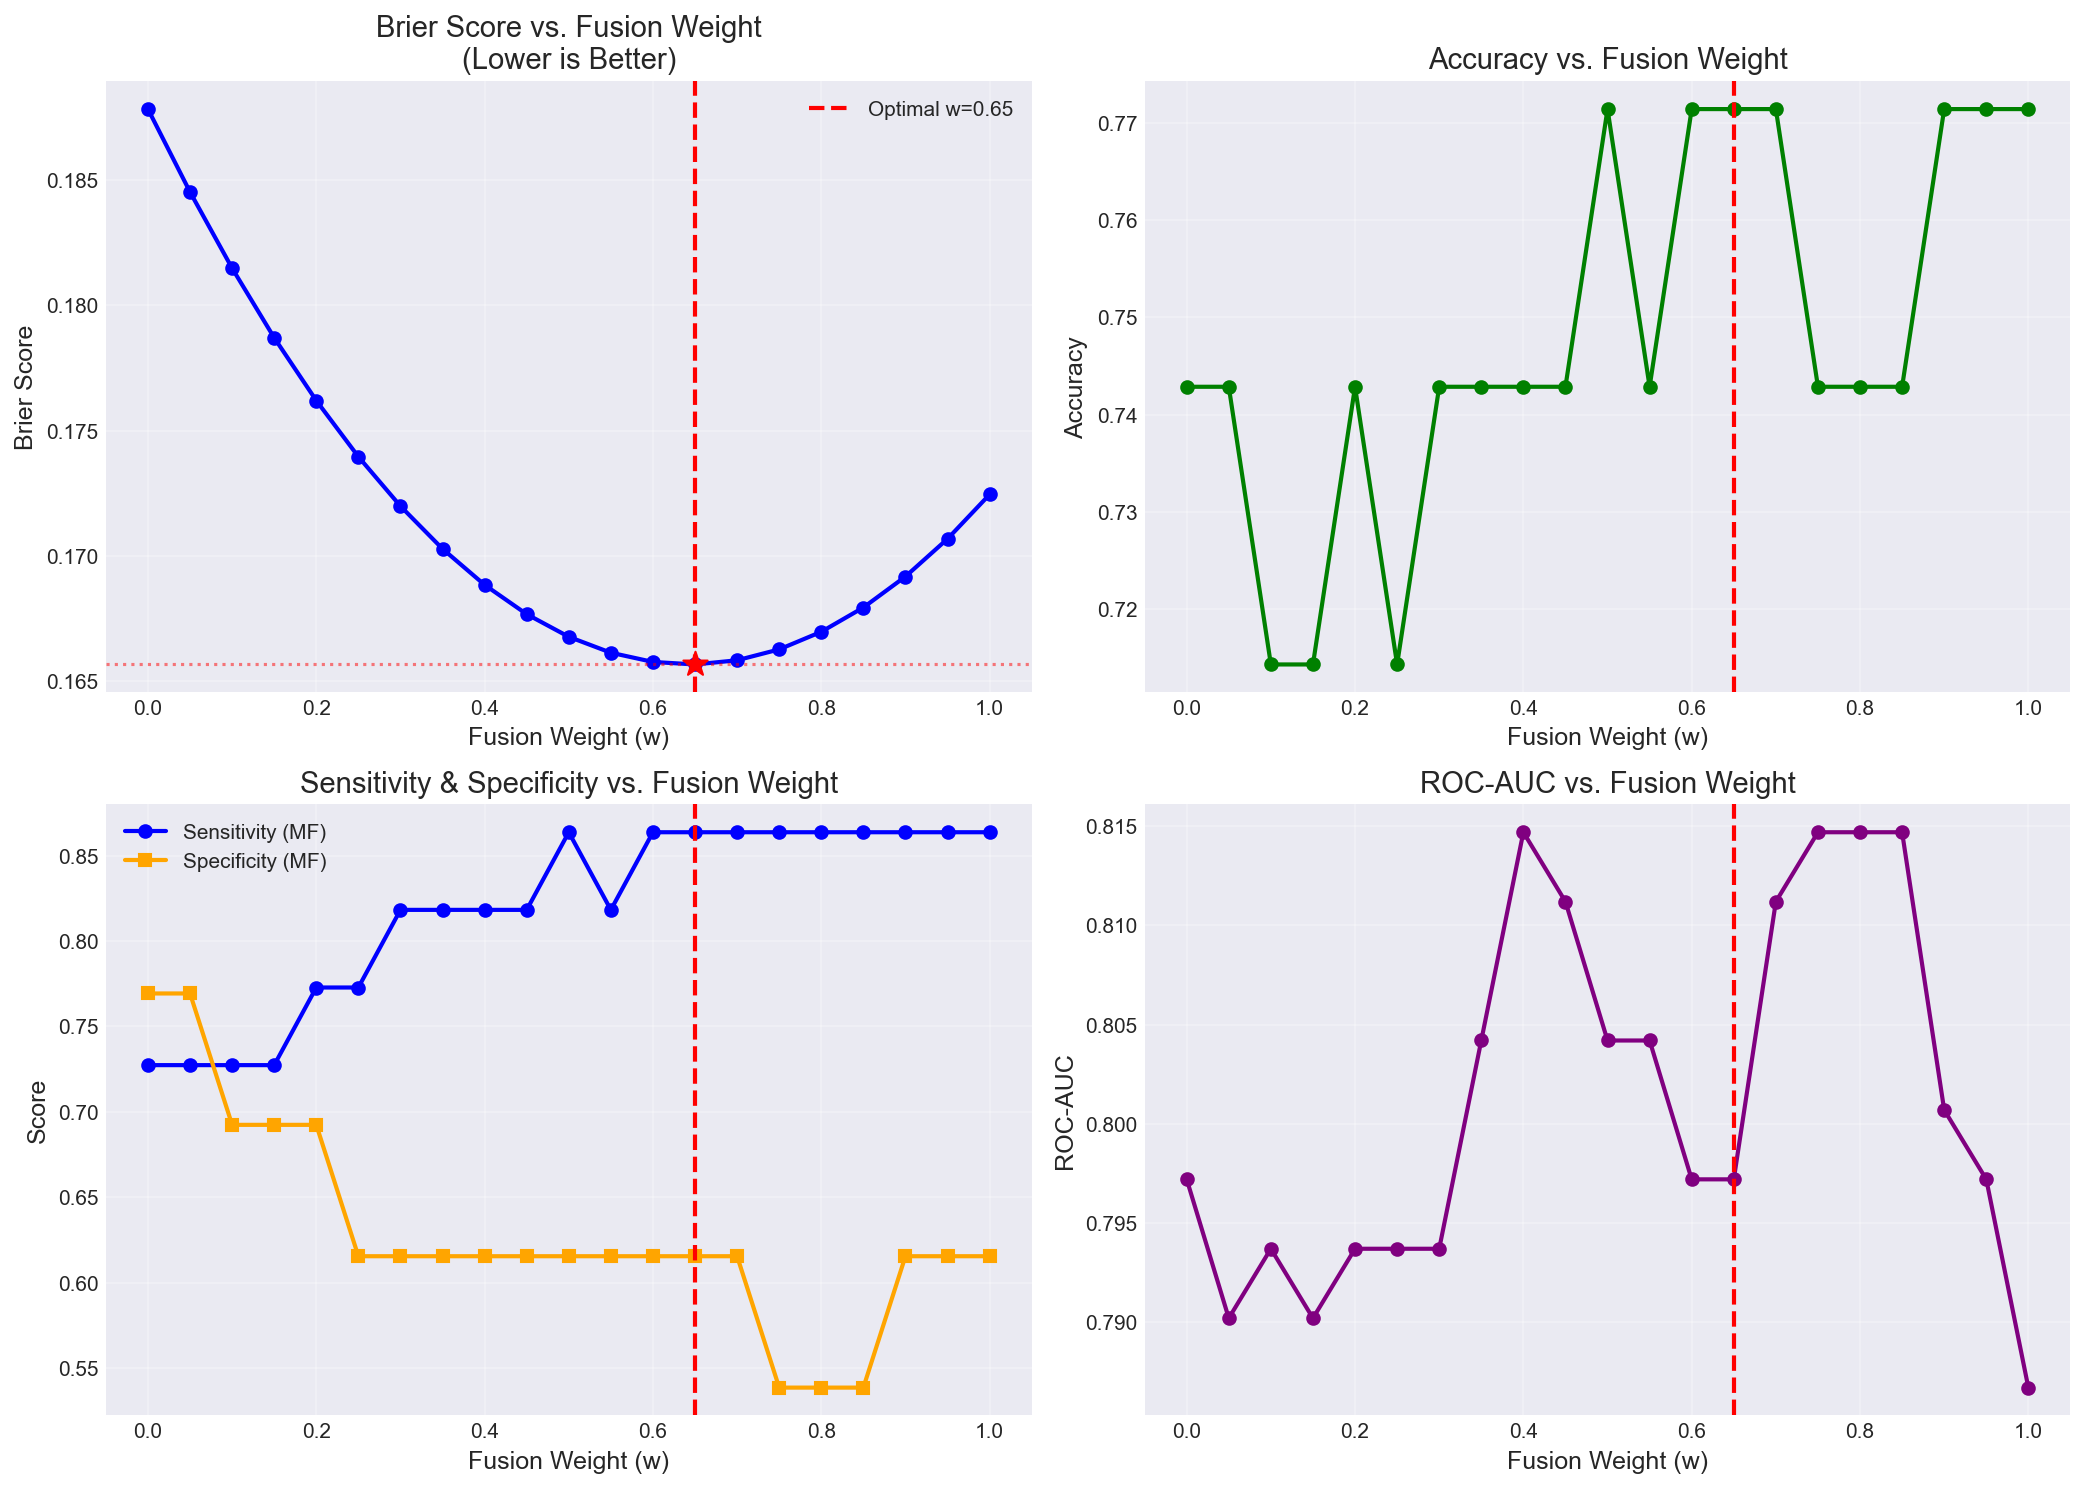
\includegraphics[width=1\linewidth]{fusion_weight_analysis.png}
    \caption{Optimization of the multi-magnification fusion weight ($\alpha$). The top-left panel demonstrates that the lowest Brier Score (indicating optimal calibration) is achieved at $\alpha=0.60$. The remaining panels illustrate the corresponding trade-offs in Accuracy, Sensitivity/Specificity, and ROC-AUC, confirming that the selected clinical weight ($\alpha=0.20$) maintains high sensitivity while maximizing predictive reliability.}
    \label{fig:fusion_analysis}
\end{figure}

\subsection{Clinical Features Classifier}
To complement the histopathological image analysis, a machine learning module was developed to evaluate structured patient metadata. A total of 16 features were selected based on univariate statistical significance and clinical relevance, encompassing demographics (e.g., age), disease history (duration, visit type, course), anatomic distribution (head/neck, lower limbs), and lesion morphology (color, macules, patches, papules, plaques, nodules, scales, and biopsy findings). 

Missing continuous values were addressed using median imputation, while categorical variables underwent label encoding. To account for class imbalance, the positive class weight was adjusted. We systematically compared three distinct algorithms using 5-fold stratified cross-validation: XGBoost (to capture non-linear feature interactions and robustness to missing data), Random Forest (for superior generalization via ensemble averaging and minimal hyperparameter sensitivity), and Logistic Regression (as a linear, probabilistic baseline). This rigorous evaluation aimed to identify the most robust complementary clinical signal for MF diagnosis.



% =====================
% 4. Results
% =====================
\section{Results}

\subsection{Deep Learning Image Analysis Results}
The proposed deep learning framework was evaluated on a held-out test set of 67 patients, comprising 12,848 patches at 10$\times$ magnification and 4,320 patches at 20$\times$ magnification. As summarized in Table \ref{tab:results}, the system achieved a maximum accuracy of 83.58\% and an F$_2$-score of 0.8874 using the late-fusion model.

\begin{table}[htbp]
\caption{Quantitative Performance Summary (Test Set, N=67 Patients)}
\label{tab:results}
\centering
\renewcommand{\arraystretch}{1.2}
\setlength{\tabcolsep}{4pt} 
\begin{tabular}{l c c c}
\toprule
 & \textbf{10$\times$ Model} & \textbf{20$\times$ Model} & \textbf{Late Fusion ($\alpha=0.20$)} \\
\midrule
Accuracy & 0.8060 & 0.8358 & \textbf{0.8358} \\
F$_2$-Score & 0.8222 & \textbf{0.8874} & \textbf{0.8874} \\
Sensitivity & 0.8043 & \textbf{0.8913} & \textbf{0.8913} \\
Specificity & 0.8043 & \textbf{0.8913} & \textbf{0.8913} \\
ROC-AUC & 0.8685 & 0.8509 & \textbf{0.8778} \\
\bottomrule
\end{tabular}
\end{table}
\subsection{Patient-Level Aggregation Benefits}
A key finding of this study is the significant performance gain achieved through patient-level aggregation. As illustrated in the comprehensive dashboard (Fig. \ref{fig:comprehensiveMetrics}), every metric improved when moving from patch-level predictions to patient-level consensus.

\begin{figure}[H]
    \centering
    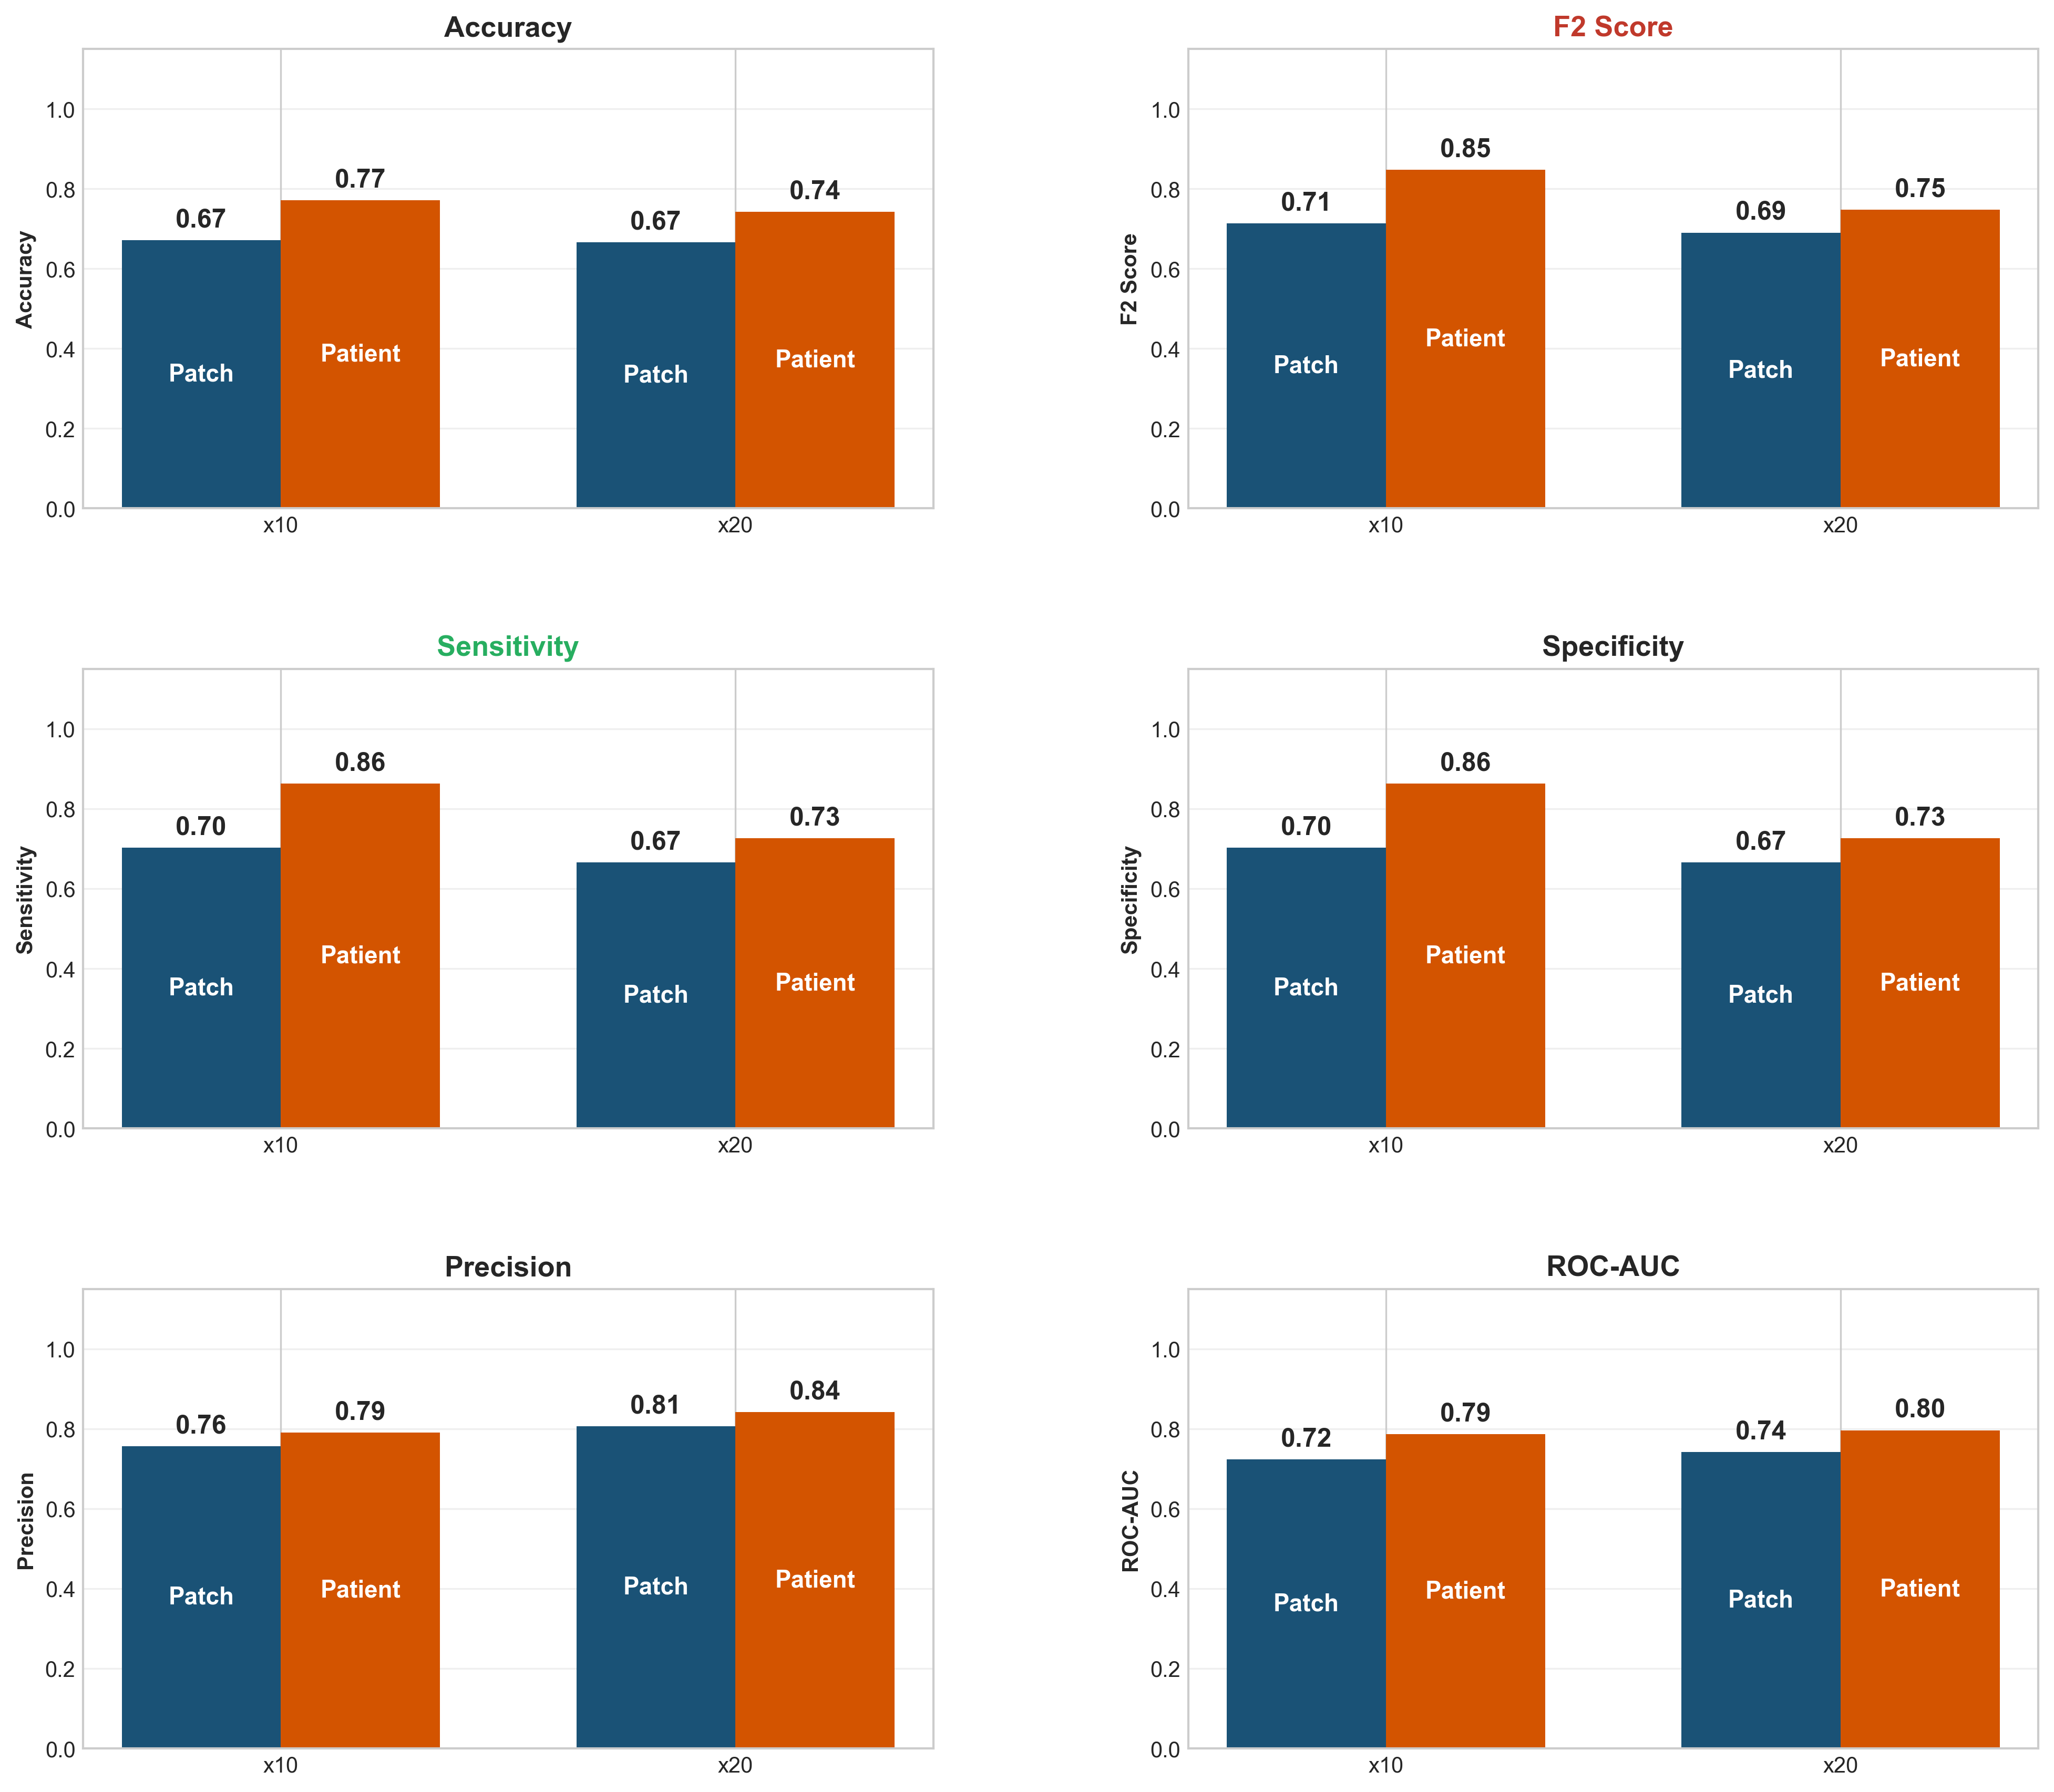
\includegraphics[width=1\linewidth]{Comprehensive Metrics Dashboard.png}
    \caption{Comprehensive Performance Dashboard. A side-by-side comparison of patch-level (dark blue) vs. patient-level (dark orange) metrics across both magnifications.}
    \label{fig:comprehensiveMetrics}
\end{figure}

\begin{figure}[H]
    \centering
    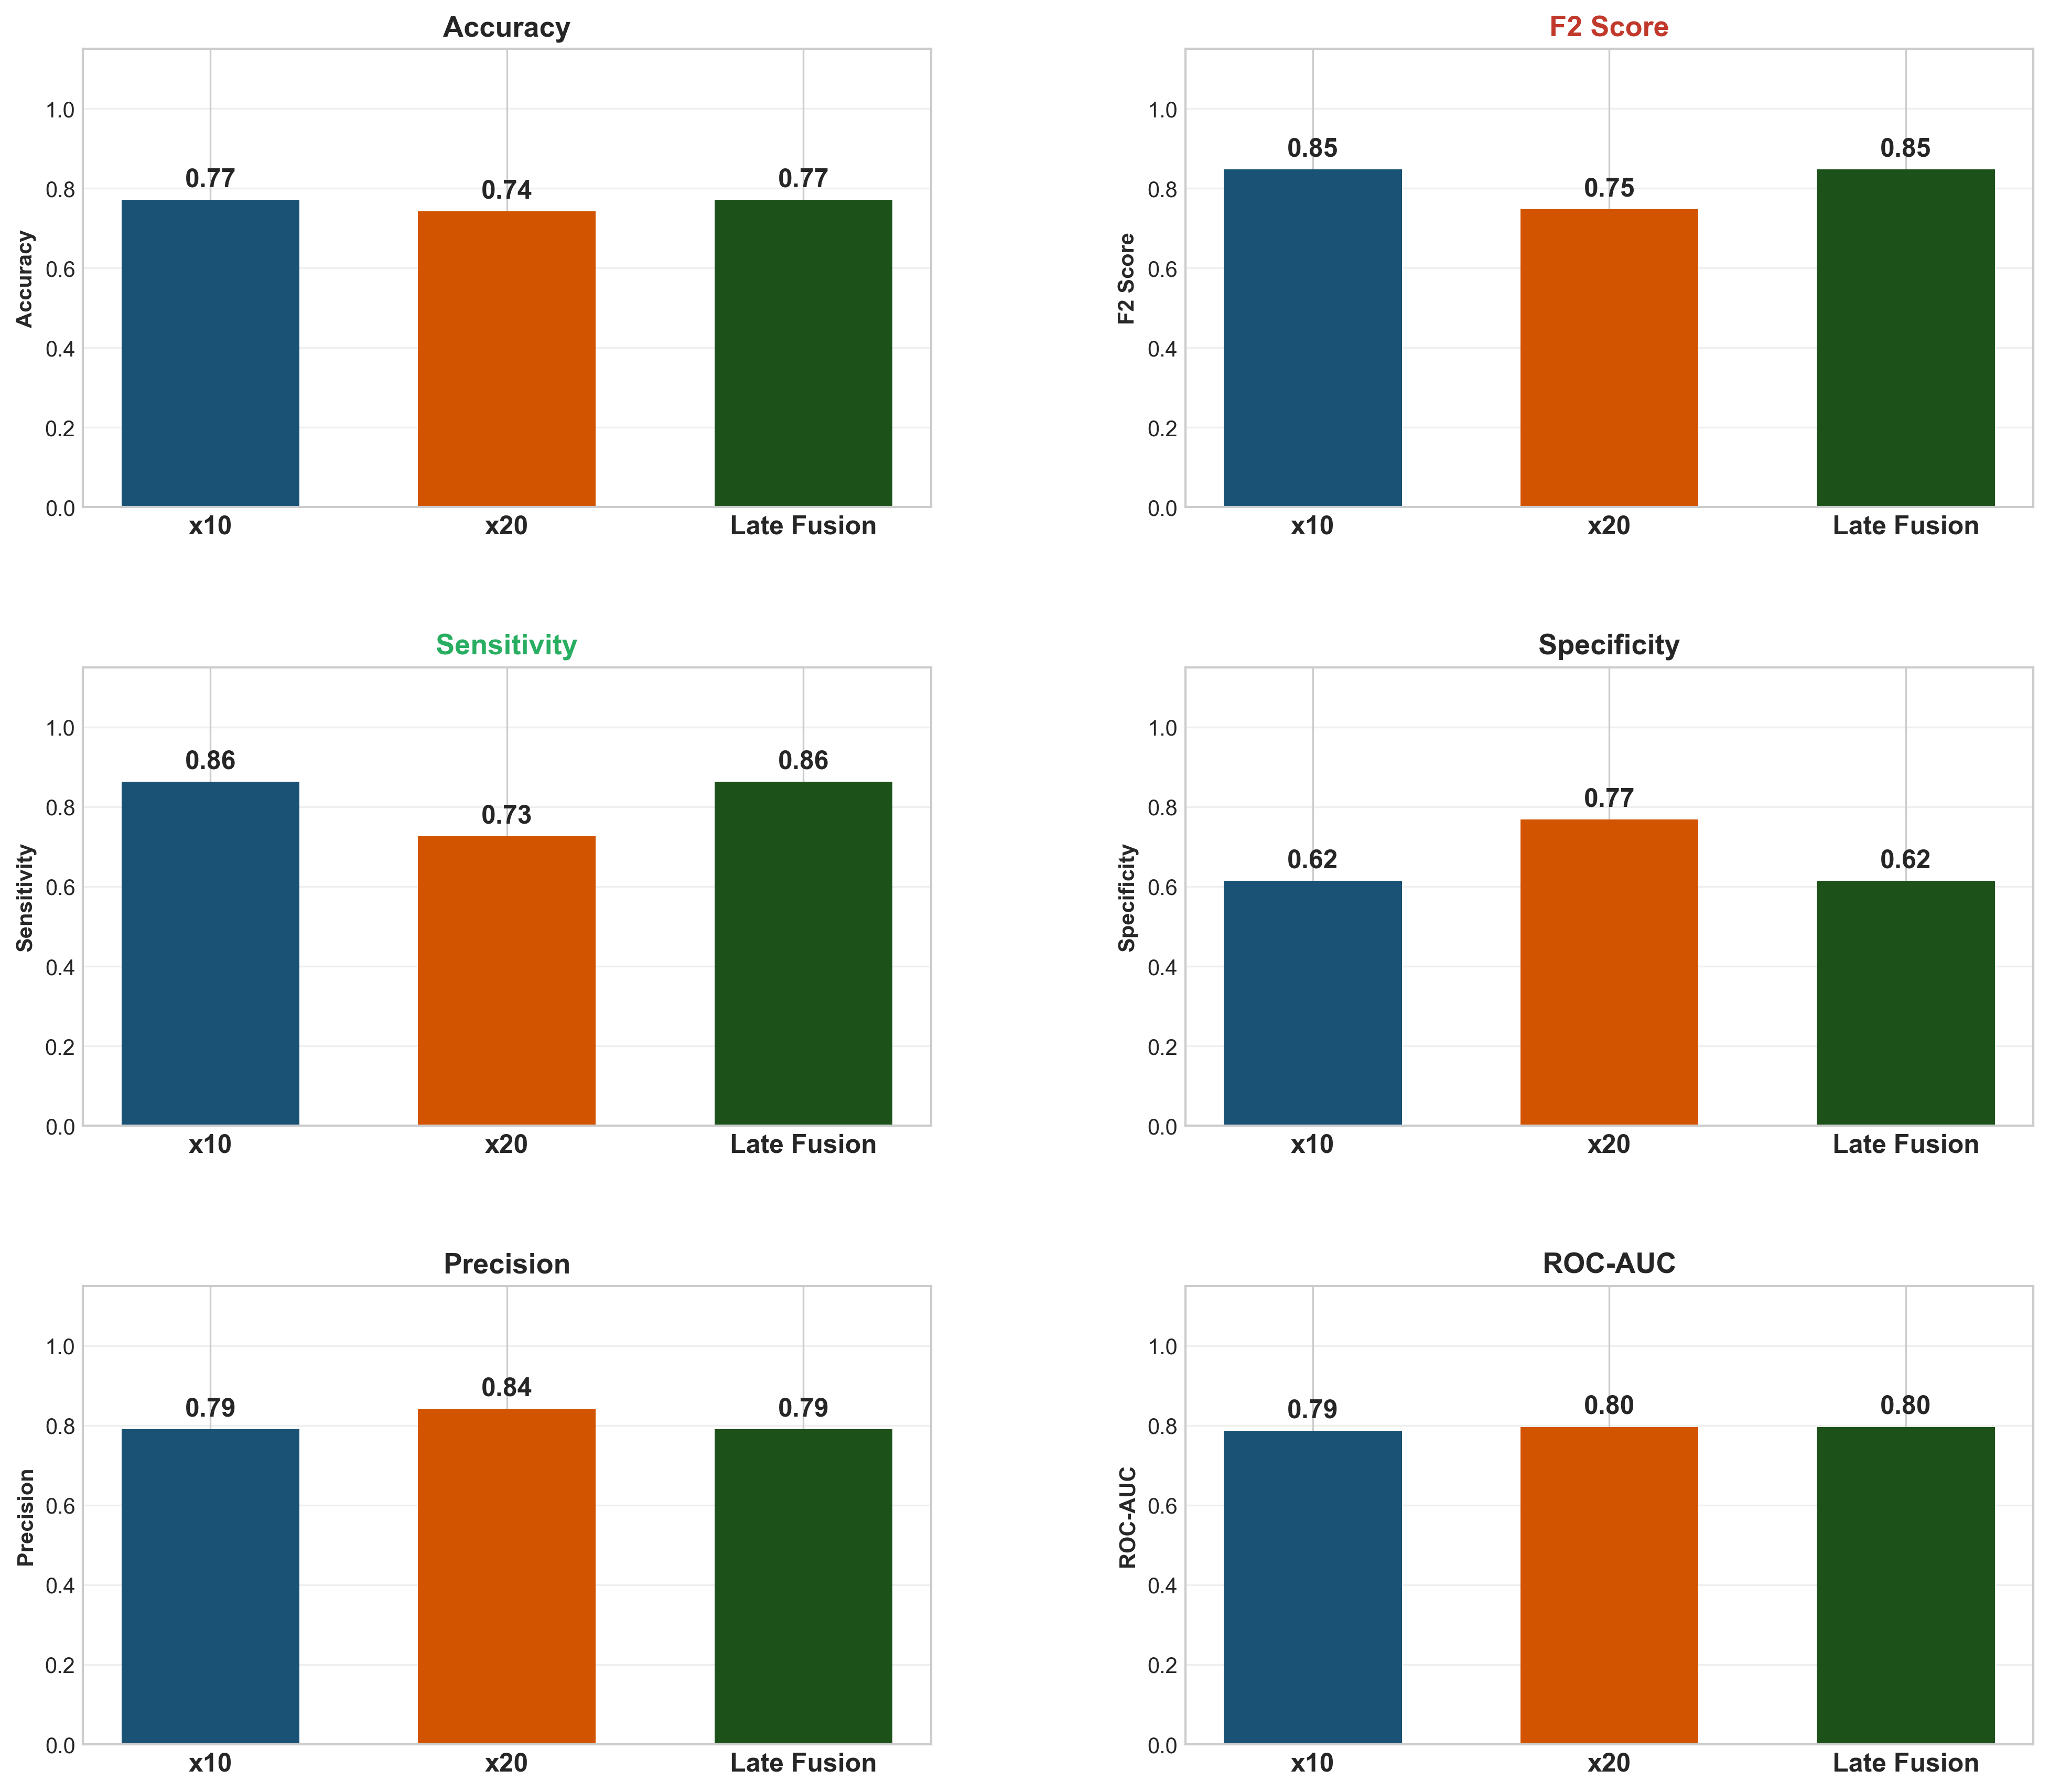
\includegraphics[width=1\linewidth]{Late_fusion_dashboard.png}
    \caption{Late fusion model performance comparing individual magnification models (10$\times$, 20$\times$) against the fused multi-scale approach. Late fusion combines predictions from both magnifications to leverage complementary information captured at different scales.}
    \label{fig:aggregation_comparison}
\end{figure}

This improvement is further detailed in the comparative performance dashboard (Fig. \ref{fig:aggregation_comparison}), which illustrates the metric shifts across magnifications and aggregation levels. The transition from patch-level to patient-level inference yields substantial gains across the board. Notably, the late fusion strategy successfully synthesizes the diagnostic strengths of both individual models: it maintains the exceptional sensitivity (0.8913) and F$_2$-score (0.8874) of the 20$\times$ patient-level model, while simultaneously maintaining a robust ROC-AUC (0.8778) and Accuracy (83.58\%). By relying heavily on the 20$\times$ model's cytological precision ($\alpha=0.20$), the late fusion effectively maximizes the detection of True Positives. In the clinical context of Mycosis Fungoides screening, prioritizing sensitivity ensures that ambiguous but potentially malignant cases are not missed, confirming the robustness of integrating detailed cellular features with broader tissue context.


\subsection{Sensitivity and Clinical Relevance}
Given the clinical imperative to minimize missed diagnoses, we prioritized the F$_2$-score (which emphasizes recall).
The 20$\times$ model achieves a superior F$_2$-score of 0.8874 compared to 0.8222 for the 10$\times$ model. This confirms that while low-power architectural changes are helpful, the high-magnification cellular details—such as hyperchromatic and cerebriform nuclei—are the most critical and discriminative indicators of MF.

\subsection{Clinical Features Classifier Results}
The clinical machine learning module demonstrated exceptional predictive power. In 5-fold stratified cross-validation on the 499 patient records, the Random Forest model emerged as the dominant classifier. As detailed in Table \ref{tab:clinical_results}, Random Forest achieved the highest Accuracy (96.6\%), Precision (94.8\%), F$_2$-Score (0.939), and ROC-AUC (0.995). While XGBoost exhibited marginally higher sensitivity (94.5\% vs 93.8\%), the Random Forest model's superior precision and overall discrimination capability established it as the optimal clinical model. Logistic Regression served as a strong linear baseline but underperformed the tree-based ensembles, highlighting the non-linear interactions within clinical presentations of MF.

\begin{table}[htbp]
\caption{Clinical Classifier Performance (5-Fold Stratified CV)}
\label{tab:clinical_results}
\centering
\renewcommand{\arraystretch}{1.2}
\setlength{\tabcolsep}{4pt} 
\begin{tabular}{l c c c}
\toprule
\textbf{Metric} & \textbf{XGBoost} & \textbf{Random Forest} & \textbf{Logistic Regression} \\
\midrule
Accuracy & 0.956 & \textbf{0.966} & 0.950 \\
Precision & 0.908 & \textbf{0.948} & 0.915 \\
Sensitivity & \textbf{0.945} & 0.938 & 0.918 \\
F$_2$-Score & 0.937 & \textbf{0.939} & 0.916 \\
ROC-AUC & 0.994 & \textbf{0.995} & 0.985 \\
\bottomrule
\end{tabular}
\end{table}

This result is corroborated by the Receiver Operating Characteristic (ROC) and Precision-Recall (PR) curves (Fig. \ref{fig:roc} and Fig. \ref{fig:pr}). The patient-level curves (solid lines) consistently envelop the patch-level curves (shaded areas), demonstrating superior discriminatory power across all decision thresholds.

\begin{figure}[H]
    \centering
    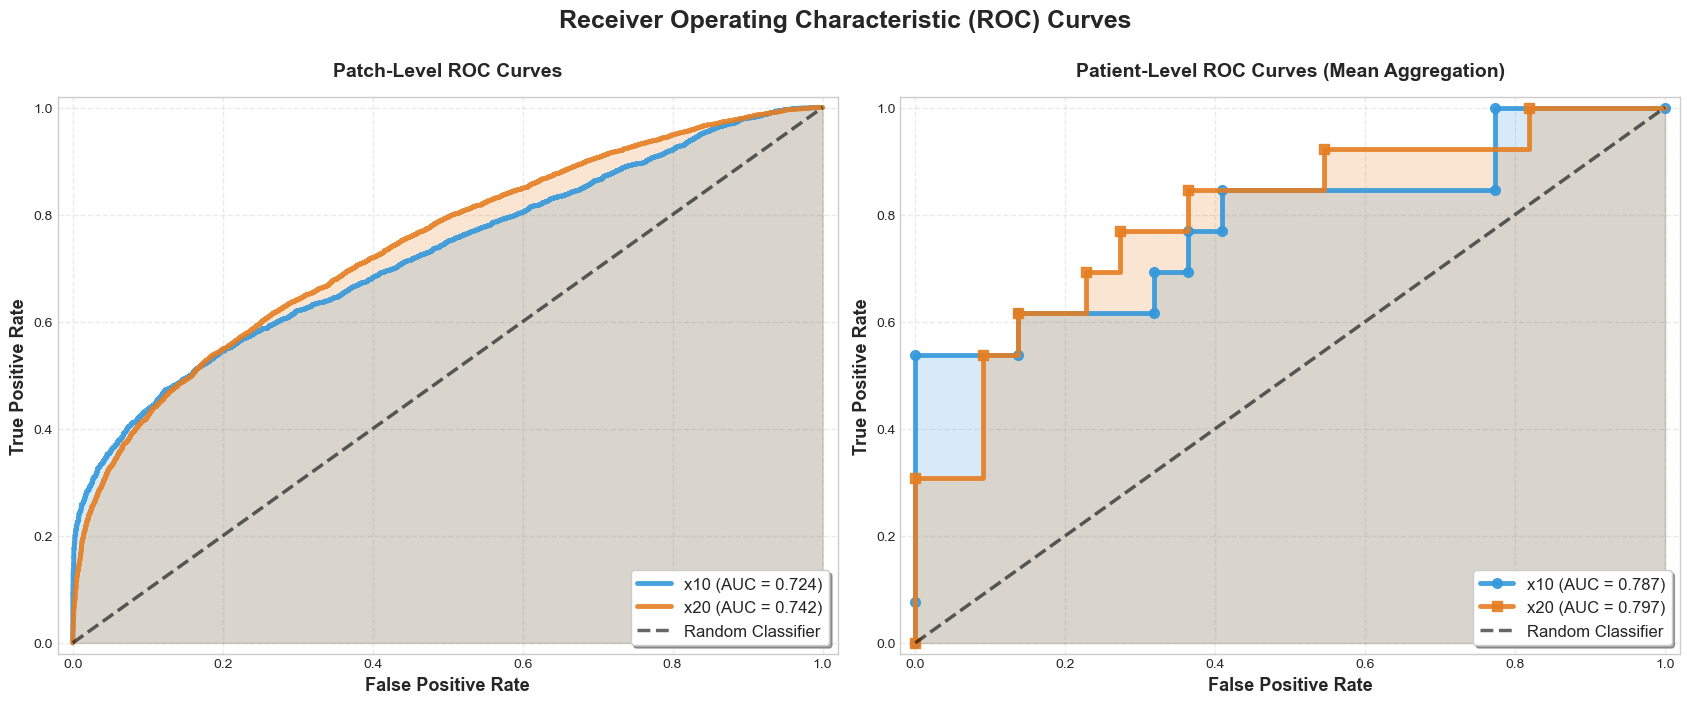
\includegraphics[width=1\linewidth]{ROC Graphs.png}
    \caption{Receiver Operating Characteristic (ROC) Curves. The "step-like" nature of the patient-level curves is due to the discrete number of test patients (N=35), yet they show a clear improvement in Area Under the Curve (AUC) compared to patch-level inference.}
    \label{fig:roc}
\end{figure}

\begin{figure}[H]
    \centering
    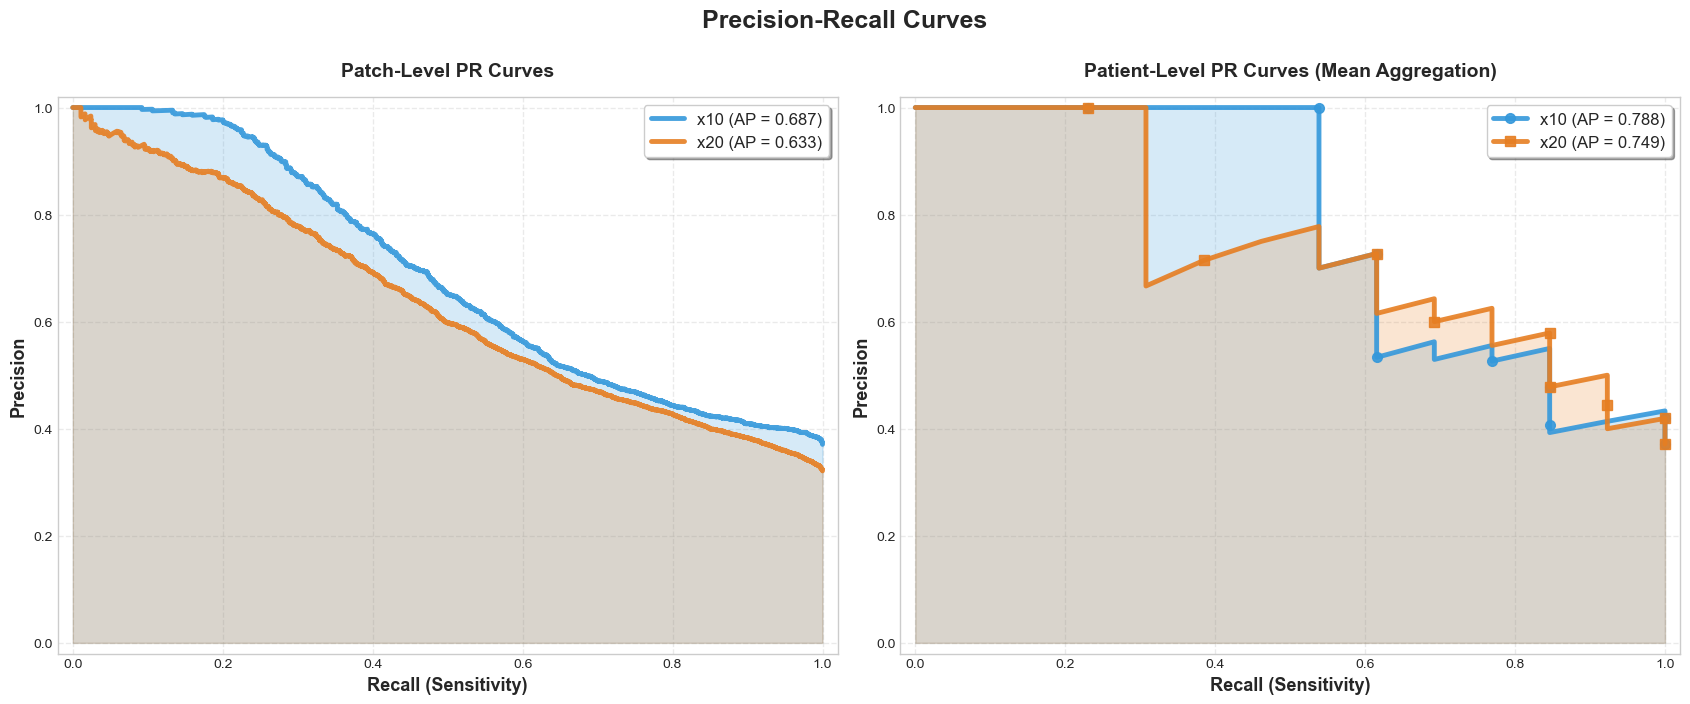
\includegraphics[width=1\linewidth]{Precision Recall Curves.png}
    \caption{Precision-Recall Curves. The dominance of the patient-level curves (solid lines) confirms that the model maintains high precision even at higher recall levels, a critical trait for a screening tool.}
    \label{fig:pr}
\end{figure}

% =====================
% 6. Discussion
% =====================
\section{Discussion}
\section{Discussion}
\subsection{Cellular Detail within Architectural Context}
A key finding of this study is the superior performance of the 20$\times$ model (F$_2$=0.8874) compared to the 10$\times$ model (F$_2$=0.8222). In histopathology, higher magnification typically yields better resolution of cellular atypia, such as hyperchromatic and irregular cerebriform nuclei, which are hallmark cytological features of Mycosis Fungoides. Our empirical results strongly support this established dermatopathologic principle, demonstrating that high-resolution cellular detail is the primary driver of accurate algorithmic diagnosis.

However, Mycosis Fungoides is also defined by architectural patterns, such as epidermotropism and the formation of Pautrier's microabscesses, which are more readily apparent at lower magnifications. Our multi-scale late-fusion approach successfully mimics the workflow of a human pathologist by combining both perspectives. By assigning 80\% of the decision weight to the 20$\times$ cytological model and 20\% to the 10$\times$ architectural model, the framework explicitly prioritizes definitive cellular evidence while still benefiting from the broader architectural context, resulting in a highly sensitive and reliable diagnostic tool.

\subsection{The Necessity of Whole-Slide Context}
The success of the patient-level aggregation strategy highlights the diffuse nature of
Mycosis Fungoides. Because MF features are rarely restricted to a few isolated "hotspots"
and are instead spread subtly across the tissue, relying on the collective signal
of the entire sample is crucial. By utilizing mean aggregation, the model effectively
integrates the probabilistic signal from all extracted patches. This approach acts as a
digital analog to a pathologist comprehensively scanning the whole tissue slide before
making a final diagnostic decision, ensuring that widespread, subtle architectural cues
are fully leveraged.
\subsection{Benchmarking and Clinical Reality}
While our deep learning framework demonstrates high diagnostic potential, it is crucial to acknowledge that diagnosing Mycosis Fungoides solely from histopathological images is a simplified proxy for clinical reality. In practice, dermatologists and pathologists rely on a multimodal synthesis of visual data, patient history, and clinical presentation (e.g., lesion morphology, duration) to render a definitive diagnosis. The reliance on image data alone in this study likely imposes a performance ceiling; we hypothesize that integrating tabular clinical metadata in future iterations will significantly enhance diagnostic precision and reduce false positives.

Despite this limitation, our model's performance is highly competitive with recent state-of-the-art benchmarks. Doeleman et al. \cite{Doeleman2024-MF} compared a weakly supervised deep learning model against three expert pathologists. They reported that their highest performance was achieved at $200\times$ magnification ($0.50$ $\mu$m/pixel), yielding a mean Area Under the Curve (AUC) of $0.827 \pm 0.044$ and a mean balanced accuracy of $76.2 \pm 3.9\%$.

In comparison, our $10\times$ model achieved a patient-level accuracy of $77.1\%$ and a sensitivity of $86.4\%$. Notably, our framework effectively matches the accuracy of expert pathologists reported in \cite{Doeleman2024-MF}.
% =====================
% 7. Conlcusion
% =====================
\section{Conclusion}
This work presents a comprehensive, multimodal machine learning framework for the automated screening of Mycosis Fungoides. By rigorously optimizing TF-EfficientNet-B3 architectures and employing a multi-scale patient-level fusion strategy, we achieved a diagnostic sensitivity of 89.13\% and an Accuracy of 83.58\% on histological images. Furthermore, by integrating a dedicated Random Forest classifier for clinical features, we demonstrated that patient metadata yields exceptional predictive accuracy (96.6\%) independently.

Our results demonstrate that prioritizing high-resolution cytological details (20$\times$) while still incorporating broad architectural context (10$\times$) yields the most robust image-based triage tool.

Our key contributions include:
\begin{enumerate}
    \item \textbf{Dominance of Cytological Details:} We proved that the 20$\times$ model's capacity to resolve fine cellular atypia significantly outperforms the broader 10$\times$ architectural view. By allocating 80\% weight to the 20$\times$ model, we maximize sensitivity, proving high magnification is critical for accurate differential diagnosis.
    
    \item \textbf{Complementary Clinical AI:} We established that a robust machine learning module analyzing just 16 structured clinical features can achieve extraordinary diagnostic performance (93.8\% sensitivity, 96.6\% accuracy). This proves that while histopathology is the gold standard, algorithmic analysis of clinical metadata is a highly reliable parallel modality.

    \item \textbf{Multi-Scale Patient-Level Late Fusion:} We designed a late-fusion protocol that integrates predictions across multiple magnifications. By systematically combining the cytological detail captured at 20$\times$ with the broader architectural context from the 10$\times$ model, our patient-level consensus approach achieved optimal performance. 
\end{enumerate}
% =====================
% 8. Discussion
% =====================
\section{Future Work}
To evolve this framework from a promising prototype into a robust clinical decision-support system, future research will address four critical limitations:

\begin{enumerate}
    \item \textbf{Deep Multimodal Fusion:} While this study developed independent deep learning and clinical machine learning models, future iterations will explore end-to-end multimodal architectures. Integrating the histopathological feature extractors directly with the clinical tabular data via cross-attention mechanisms is expected to yield a unified model that surpasses the performance of the independent branches.

    \item \textbf{Stain Normalization and Augmentation:} To ensure the model generalizes across different laboratories and scanners, we will implement rigorous stain normalization techniques (e.g., Macenko \cite{macenko2009} or Vahadane \cite{vahadane2016_stainnorm} methods) in the preprocessing pipeline. This will mitigate the impact of color variations in H\&E staining that can currently confound the classifier.

\end{enumerate}


\bibliographystyle{IEEEtran}
\bibliography{references}

\vspace{12pt}


\end{document}
